
Coroutines are functions that can suspend their execution and resume it later on. They allow writing asynchronous code in a very similar manner to how you would write synchronous code. Compared to writing asynchronous code with std::async, this allows writing cleaner code that's easier to understand and maintain. There's no need to write callbacks anymore, and no need to deal with the verbosity of std::async with promises and futures.

Aside from all that, they can also often provide you with much better performance. std::async based code usually has more overhead for switching threads and waiting. Coroutines can resume and suspend very cheaply even compared to the overhead of calling functions, which means they can yield better latency and throughput. Also, one of their design goals was to be highly scalable, even to billions of concurrent coroutines.

\begin{center}
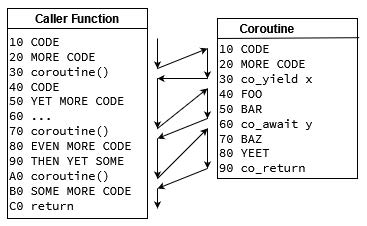
\includegraphics[width=0.9\textwidth]{content/3/chapter11/images/1.jpg}\\
Figure 11.1 – Calling and executing coroutines is different from using regular functions as they can be suspended and resumed
\end{center}

C++ coroutines are stackless, which means their state is not stored on the calling thread's stack. This gives them an interesting property: several different threads can pick up the execution of a coroutine. In other words, even though it looks like the coroutine function body would be executed sequentially, parts of it can be executed in different threads. This makes it possible to leave parts of the function to be executed on dedicated threads. For instance, I/O operations can be done in a dedicated I/O thread.

To check whether a function is a C++ coroutine, you need to look for one of the following keywords in its body:

\begin{itemize}
\item 
co\_await, which suspends the coroutine.

\item 
co\_yield for returning a value to the caller and suspending the coroutine.

\item 
Similar to Python's yield keyword used in generators. Allows generating values lazily.

\item 
co\_return, which returns a value and finishes executing the coroutine. It's a coroutine equivalent of the return keyword.
\end{itemize}

Whenever a function body has one of those keywords, the function automatically becomes a coroutine. Although this means it's an implementation detail, there's one more hint that you can use: coroutine return types must satisfy certain requirements, which we'll discuss later on.

Coroutines are first-class citizens in the C++ world. This means you can get their address, use them as function arguments, return them from functions, and store them in objects.

In C++, you could write coroutines even before C++20. This was possible thanks to libraries such as Boost.Coroutine2, or Bloomberg's Quantum. The latter was even used to implement CoroKafka – a library for efficiently dealing with Kafka streams using coroutines. With the advent of standard C++ coroutines, new libraries started popping up. Now, we're going to show you one of them.

\subsubsubsection{11.5.1\hspace{0.2cm}Distinguishing between cppcoro utilities}

It's hard to write coroutine-based code from scratch. C++20 only offers the fundamental utilities for writing coroutines, so we need a set of primitives to use when writing our own coroutines. The cppcoro library created by Lewis Baker is one of the most commonly used coroutine frameworks for C++. In this section, we'll showcase the library and demonstrate how to use it when writing coroutine-based code.

Let's start with an overview of the coroutine types the library offers us:

\begin{itemize}
\item 
task<>: For scheduling work to be executed later – starts executing when it's co\_awaited for.

\item 
shared\_task<>: A task that multiple coroutines can await. It can be copied so that multiple coroutines reference the same result. Doesn't offer any thread-safety on its own.

\item 
generator: Produces a sequence of Ts lazily and synchronously. It's effectively a std::range: it has a begin() returning an iterator and an end() returning a sentinel.

\item 
recursive\_generator: Similar to generator<T>, but can yield either a T or recursive\_generator<T>. Has some extra overhead.

\item 
async\_generator: Similar to generator<T>, but values may be produced asynchronously. This means that, as opposed to generator, asynchronous

\item 
generators can use co\_await in their bodies.
\end{itemize}

You should use those types as return types for your coroutines. Usually, in your generators (coroutines returning one of the preceding generator types), you'd want to return values using co\_yield (similar to in Python generators). In your tasks, however, usually, you'll want to schedule work with co\_await.

The library actually offers many more programming abstractions than just the preceding coroutine types. It also provides the following types:

\begin{itemize}
\item 
Awaitables types that you can co\_await on, such as coroutine-flavored events and synchronization primitives: mutexes, latches, barriers, and so on.

\item 
Cancellation-related utilities, essentially allowing you to cancel the execution of your coroutines.

\item 
Schedulers – objects allowing you to schedule work through them, such as static\_thread\_pool, or ones for scheduling work on a specific thread.

\item 
I/O and networking utilities, allowing you to read from and write to files and IP sockets.

\item 
Meta-functions and concepts, such as awaitable\_traits, Awaitable, and Awaiter.
\end{itemize}

Aside from the preceding utilities, cppcoro offers us functions – utilities for using other classes and steering execution, such as the following:

\begin{itemize}
\item 
sync\_wait: Block until the passed awaitable completes.

\item
when\_all, when\_all\_ready: Return an awaitable that completes when all the passed awaitables complete. The difference between those two is in handling failures of the sub-awaitables. when\_all\_ready will complete even in the event of failures and the caller can examine each result, while when\_all will rethrow an exception if any of the sub-awaitables throws one (it's impossible to know which one did, though). It will also cancel any incomplete tasks.

\item
fmap: Similarly to functional programming, applies a function to an awaitable. You can think of it as transforming a task of one type into a task of another. For example, you can serialize types returned by your coroutines by calling fmap(serialize, my\_coroutine()).

\item
resume\_on: Instructs the coroutine which scheduler to use to continue execution once some work is completed. This enables you to execute certain work in certain execution contexts, such as running I/O-related tasks on a dedicated I/O thread. Note that this means a single C++ function (coroutine) can execute its parts on separate threads. Can be "piped" with computations similarly to std::ranges.

\item
schedule\_on: Instructs the coroutine which scheduler to use to start some work. Commonly used as auto foo = co\_await schedule\_on(scheduler,
do\_work());.
\end{itemize}

Before we start using those utilities together, let's say a few more words about awaitables.

\subsubsubsection{11.5.2\hspace{0.2cm}Looking under the hood of awaitables and coroutines}

Aside from cppcoro, the standard library offers two more trivial awaitables: suspend\_never and suspend\_always. By looking at them, we can see how to implement our own awaitables when needed:

\begin{lstlisting}[style=styleCXX]
struct suspend_never {
	constexpr bool await_ready() const noexcept { return true; }
	constexpr void await_suspend(coroutine_handle<>) const noexcept {}
	constexpr void await_resume() const noexcept {}
};

struct suspend_always {
	constexpr bool await_ready() const noexcept { return false; }
	constexpr void await_suspend(coroutine_handle<>) const noexcept {}
	constexpr void await_resume() const noexcept {}
};
\end{lstlisting}

When typing co\_await, you tell the compiler to first call the awaiter's await\_ready(). If it says the awaiter is ready by returning true, await\_resume() will get called. The return type of await\_resume() should be the type the awaiter is actually producing. If the awaiter was not ready, the program will instead execute await\_suspend(). After it's done, we have three cases:

\begin{itemize}
\item 
await\_suspend returns void: The execution will always suspend afterwards.

\item 
await\_suspend returns bool: The execution will suspend or not depending on the returned value.

\item 
await\_suspend returns std::coroutine\_handle<PromiseType>: Another coroutine will get resumed.
\end{itemize}

There's much more going on with coroutines under the hood. Even though coroutines don't use the return keyword, the compiler will generate code under the hood to make them compile and work. When using keywords such as co\_yield, it will rewrite them to calls to the appropriate member functions of helper types. For instance, a call to co\_yield x is equivalent to co\_await promise.yield\_value(x). If you want to learn more about what's happening exactly and write your own coroutine types, refer to the Your First Coroutine article from the Further reading section.

Okay, let's now use all this knowledge to write our own coroutines. We'll create a simple application that mimics doing meaningful work. It will use a thread pool to fill a vector with some numbers.

Our CMake target will look as follows:

\begin{lstlisting}[style=styleCMake]
add_executable(coroutines_1 coroutines/main_1.cpp)
target_link_libraries(coroutines_1 PRIVATE cppcoro fmt::fmt
Threads::Threads)
target_compile_features(coroutines_1 PRIVATE cxx_std_20)
\end{lstlisting}

We'll link to the cppcoro library. In our case, we're using Andreas Buhr's fork of cppcoro, as it is a well-maintained fork of Lewis Baker's repository and supports CMake. 

We'll also link to the excellent \{fmt\} library for text formatting. If your standard library offers C++20's string formatting, you can use that instead.

Last but not least, we're going to need a threading library – after all, we want to use multiple threads in a pool.

Let's start our implementation with some constants and a main function:

\begin{lstlisting}[style=styleCXX]
inline constexpr auto WORK_ITEMS = 5;

int main() {
	auto thread_pool = cppcoro::static_thread_pool{3};
\end{lstlisting}

We want to produce five items using three pooled threads. cppcoro's thread pool is a neat way to schedule work. By default, it creates as many threads as your machine has hardware ones. Moving onward, we need to specify our work:

\begin{lstlisting}[style=styleCXX]
fmt::print("Thread {}: preparing work\n", std::this_thread::get_id());
auto work = do_routine_work(thread_pool);

fmt::print("Thread {}: starting work\n", std::this_thread::get_id());
const auto ints = cppcoro::sync_wait(work);
\end{lstlisting}

We'll sprinkle our code with log messages so you can better see what's going on in which thread. This will help us better understand how coroutines work. We create work by calling a coroutine named do\_routine\_work. It returns us the coroutine, which we run using the sync\_wait blocking function. A coroutine won't start executing until it is actually being awaited. This means that our actual work will start inside this function call.

Once we have our results, let's log them:

\begin{lstlisting}[style=styleCXX]
fmt::print("Thread {}: work done. Produced ints are: ",
			std::this_thread::get_id());
for (auto i : ints) {
	fmt::print("{}, ", i);
}
fmt::print("\n");
\end{lstlisting}

No voodoo magic here. Let's define our do\_routine\_work coroutine:

\begin{lstlisting}[style=styleCXX]
cppcoro::task<std::vector<int>>
do_routine_work(cppcoro::static_thread_pool &thread_pool) {
	auto mutex = cppcoro::async_mutex{};
	auto ints = std::vector<int>{};
	ints.reserve(WORK_ITEMS);
\end{lstlisting}

It returns a task, which produces some integers. Because we're going to use the thread pool, let's use cppcoro's async\_mutex to synchronize the threads. Let's now start using the pool:

\begin{lstlisting}[style=styleCXX]
fmt::print("Thread {}: passing execution to the pool\n",
			std::this_thread::get_id());
co_await thread_pool.schedule();
\end{lstlisting}

You might be surprised that the schedule() call doesn't pass in any callable to execute. In the coroutine's case, we're actually making our current thread suspend the coroutine and start executing its caller. This means it will now wait for the coroutine to finish (somewhere in the sync\_wait call).

In the meantime, a thread from our pool will resume the coroutine – simply continuing to execute its body. Here's what we've prepared for it:

\begin{lstlisting}[style=styleCXX]
fmt::print("Thread {}: running first pooled job\n",
			std::this_thread::get_id());
			
std::vector<cppcoro::task<>> tasks;
for (int i = 0; i < WORK_ITEMS; ++i) {
	tasks.emplace_back(
		cppcoro::schedule_on(thread_pool, fill_number(i, ints, mutex)));
}
co_await cppcoro::when_all_ready(std::move(tasks));
co_return ints;
\end{lstlisting}

We create a vector of tasks to execute. Each task fills one number in ints under the mutex. The schedule\_on call runs the filling coroutine using another thread from our pool. Finally, we wait for all the results. At this point, our tasks start executing. Finally, as our coroutine is a task, we use co\_return .

\begin{tcolorbox}[colback=blue!5!white,colframe=blue!75!black, title=Note]
\hspace*{0.7cm}Don't forget to co\_return the produced value. If we removed the co\_return ints; line from our example, we would simply return a default constructed vector. The program would run, happily print the empty vector, and exit with code 0.
\end{tcolorbox}

Our last step is to implement the coroutine that will produce a number:

\begin{lstlisting}[style=styleCXX]
cppcoro::task<> fill_number(int i, std::vector<int> &ints,
cppcoro::async_mutex &mutex) {
	fmt::print("Thread {}: producing {}\n", std::this_thread::get_id(), i);
	std::this_thread::sleep_for(
		std::chrono::milliseconds((WORK_ITEMS - i) * 200));
\end{lstlisting}

This one is a task that doesn't return any value. Instead, it will add it to our vector. Its hard work will actually be done by dozing off for a number of milliseconds. After the wake-up, the coroutine will continue with more productive endeavors:

\begin{lstlisting}[style=styleCXX]
{
	auto lock = co_await mutex.scoped_lock_async();
	ints.emplace_back(i);
}
\end{lstlisting}

It will lock the mutex. In our case, it's just an await. When the mutex is locked, it will add a number to our vector – the same number it was called with.

\begin{tcolorbox}[colback=blue!5!white,colframe=blue!75!black, title=Note]
\hspace*{0.7cm}Remember to co\_await. If you forget and your awaitable allows that (perhaps because its okay to not consume each awaitable), then you might skip some essential computations. In our example, this could mean not locking a mutex.
\end{tcolorbox}

Let's finish the coroutine's implementation now:

\begin{lstlisting}[style=styleCXX]
 fmt::print("Thread {}: produced {}\n", std::this_thread::get_id(), i);
co_return;
\end{lstlisting}

Just a simple status print and a co\_return to mark the coroutine as complete. Once it returns, the coroutine frame can be destroyed, freeing the memory occupied by it.

That's all. Let's now run our code and see what happens:

\begin{tcblisting}{commandshell={}}
Thread 140471890347840: preparing work
Thread 140471890347840: starting work
Thread 140471890347840: passing execution to the pool
Thread 140471890282240: running first pooled job
Thread 140471890282240: producing 4
Thread 140471881828096: producing 1
Thread 140471873373952: producing 0
Thread 140471890282240: produced 4
Thread 140471890282240: producing 3
Thread 140471890282240: produced 3
Thread 140471890282240: producing 2
Thread 140471881828096: produced 1
Thread 140471873373952: produced 0
Thread 140471890282240: produced 2
Thread 140471890347840: work done. Produced ints are: 4, 3, 1, 0, 2,
\end{tcblisting}

Our main thread was used to fire up the work on the pool and then waited for the results to come. Then, our three threads from the pool were producing numbers. The last task scheduled was actually the first one that ran, producing the number 4. This is because it was the one that continued executing do\_routine\_work all the time: first, it scheduled all other tasks on the pool, then started performing the first task when when\_all\_ready was called. Later on, the execution continued with the first free thread taking the next task scheduled on the pool until the whole vector was filled. Finally, the execution returned to our main thread.

This concludes our short example. And with it, we conclude our last section of this chapter. Let's now summarize what we've learned.


